\famichapter{Introduction}{This chapter introduces FamiPet, a pet-care and adoption
platform. It describes the purpose of the project, the scope of this black book, the
overall system context, and the document structure.}{ch:intro}

\section{Project Overview}

FamiPet is a full-stack web application that supports pet owners, prospective
adopters, and platform administrators. The application lets registered users
maintain profiles for their pets, generate a digital pet identity with a QR code,
record health and vaccination information, book veterinary appointments, set
medication and care reminders, participate in a community, report lost or found
animals, and apply to adopt pets listed on the platform. An administrator can
moderate content, manage users, and process adoption requests.

The system is built as a client--server application. The backend is a Node.js~\cite{nodejs}
application written with Express~\cite{express} that exposes a REST API and persists all data in
MongoDB through the Mongoose object-document mapper. The frontend is a React and
TypeScript web application built with Vite and Tailwind CSS; it communicates with
the backend over HTTP, and the backend remains the source of truth for all data
and business rules.

\section{Purpose of this Document}

This black book is a formal academic record of the FamiPet project. It documents,
from the actual implementation:

\begin{itemize}
    \item the problem the project addresses and its objectives;
    \item the functional and non-functional requirements and the system scope;
    \item the analysis and design of the system;
    \item the system architecture and deployment;
    \item the data model stored in MongoDB;
    \item the authentication, authorization, and security mechanism;
    \item the core features and their workflows;
    \item the implementation structure and technology stack;
    \item the testing performed and its evidence;
    \item the development process followed;
    \item conclusions and future work.
\end{itemize}

Every statement about behaviour, data, security, and testing in this document is
derived from the verified implementation in the repository. Planned work, such as
the remaining roadmap phases described in Chapter~\ref{ch:conclusion}, is
explicitly identified as planned rather than as delivered functionality.

\section{System Context}

Figure~\ref{fig:system-context} shows the context of the system. The backend API
is the central component: it receives HTTP requests from the frontend, applies
authentication and ownership rules, and persists and retrieves data in MongoDB.
It also integrates with external services for e-mail delivery, AI-powered pet
care assistance, and image processing.

\begin{figure}[htbp]
    \centering
    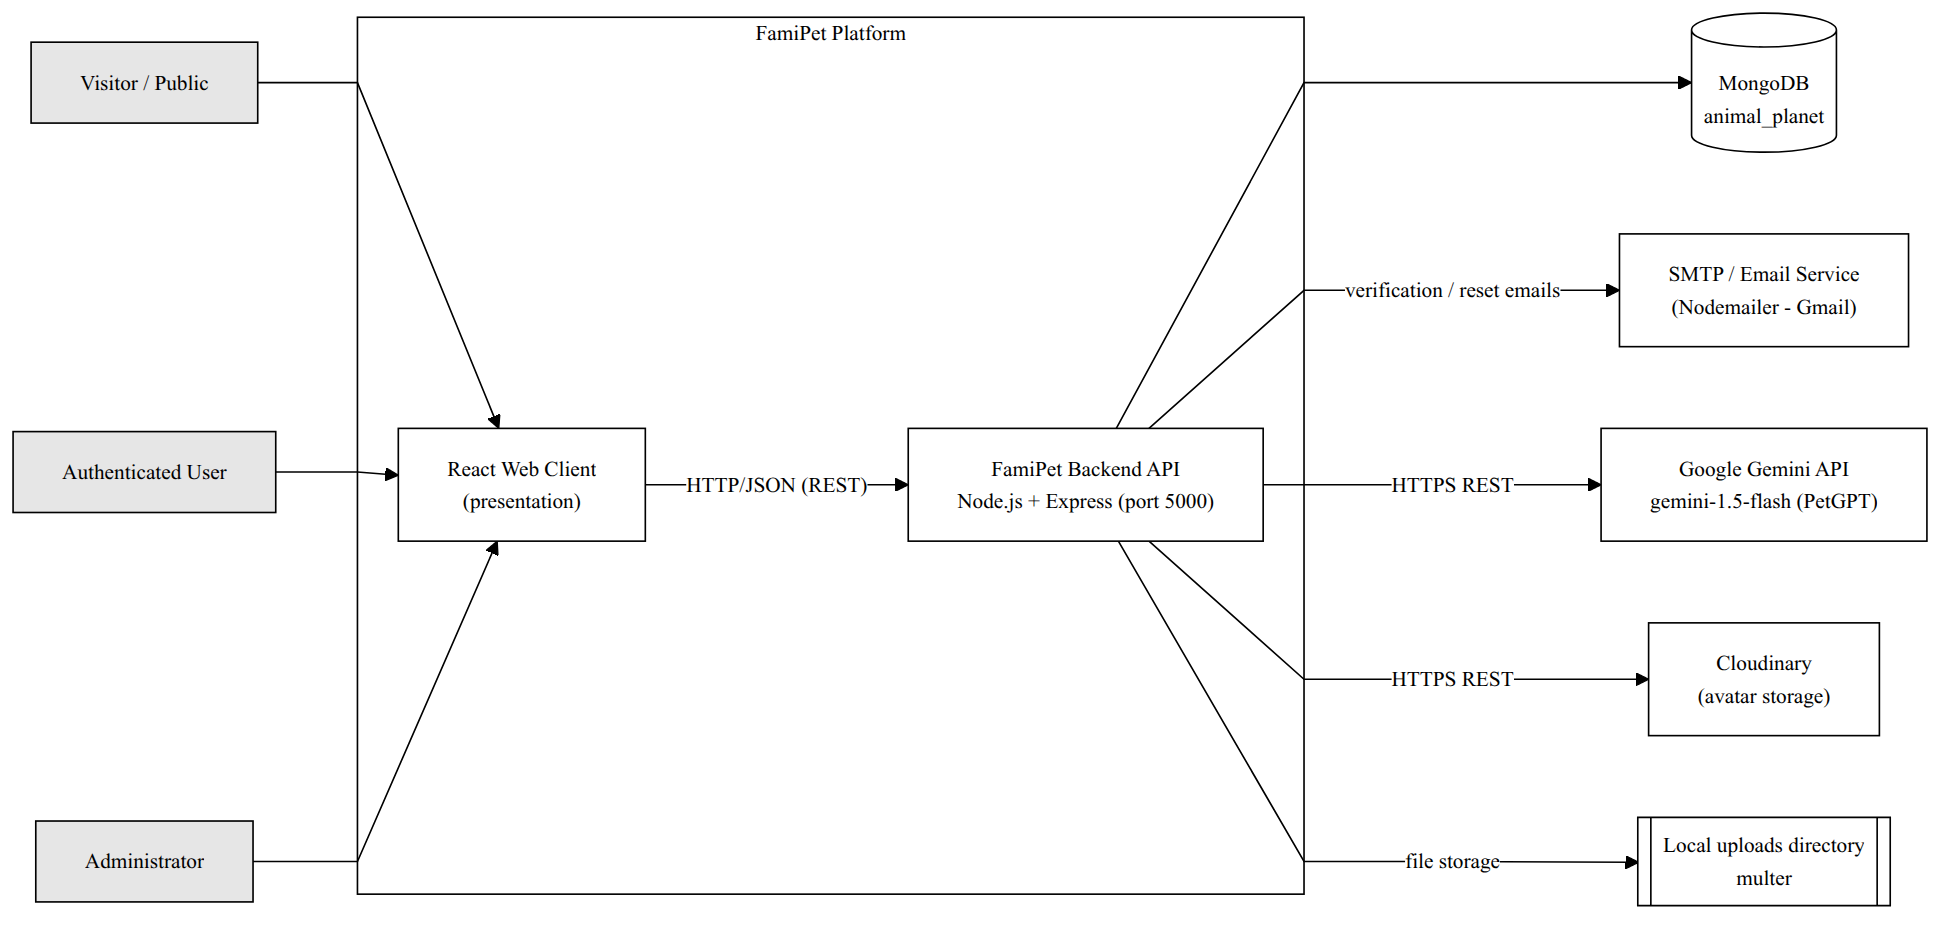
\includegraphics[width=\textwidth]{figures/01-system-context.png}
    \caption{FamiPet system context diagram.}
    \label{fig:system-context}
\end{figure}

The context diagram shows four external parties. The \emph{React web client}
interacts with the platform through the public HTTP API; the \emph{MongoDB}
database stores
all records; the \emph{e-mail service} (Nodemailer over SMTP) delivers account
verification and password-reset messages; and the \emph{Google Gemini} AI service
provides the conversational pet-care assistant. Uploaded images are stored on
Cloudinary when credentials are configured and served locally from the
\texttt{uploads} directory otherwise.

\section{Document Structure}

The black book is organised as follows. Chapter~2 defines the problem and
objectives. Chapter~3 presents the requirement specification and scope, including
functional and non-functional requirements, user roles, and use cases.
Chapter~4 analyses the system and the technology stack. Chapter~5 describes the
architecture and design. Chapter~6 documents the MongoDB data model. Chapter~7
describes authentication, authorization, and security. Chapter~8 explains the
core features and their workflows. Chapter~9 describes the implementation
structure. Chapter~10 records the testing and validation evidence. Chapter~11
documents the development process. Chapter~12 presents the conclusion and future
scope. The list of terms and abbreviations appears before the main matter;
references and two appendices conclude the black book.